\documentclass{standalone}

\usepackage{circuitikz}

\begin{document}

% INT_AY20_MP2_L29_Fig02-Attracting_masses.png

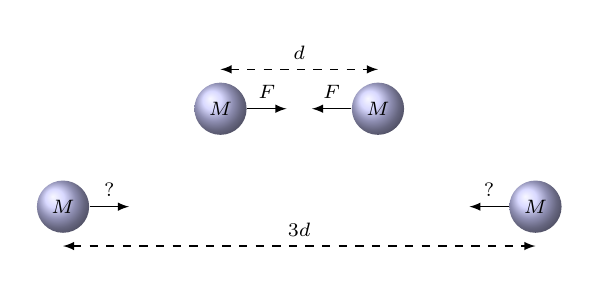
\begin{tikzpicture}[> = latex, font = \scriptsize]
	
	\matrix[row sep = 0.5 cm]{
	
		% Masses close together
		
		\node (close1) [circle, ball color = blue!20] at (-1, 0) {$M$};
		\node (close2) [circle, ball color = blue!20] at (1, 0) {$M$};
		
		% Vectors for forces
		
		\begin{scope}[->]
		
			\draw (close1.east) -- node [midway, above] {$F$} ++ (0.5, 0);
			\draw (close2.west) -- node [midway, above] {$F$} ++ (-0.5, 0);
		
		\end{scope}
		
		% Distance indicator
		
		\draw [<->, dashed] (-1, 0.5) -- node [midway, above] {$d$} (1, 0.5);

	\\
	
		% Masses far apart
		
		\node (close1) [circle, ball color = blue!20] at (-3, 0) {$M$};
		\node (close2) [circle, ball color = blue!20] at (3, 0) {$M$};
		
		% Vectors for forces
		
		\begin{scope}[->]
		
			\draw (close1.east) -- node [midway, above] {?} ++ (0.5, 0);
			\draw (close2.west) -- node [midway, above] {?} ++ (-0.5, 0);
		
		\end{scope}
		
		% Distance indicator
		
		\draw [<->, dashed] (-3, -0.5) -- node [midway, above] {$3d$} (3, -0.5);
		
	\\
	};

\end{tikzpicture}

\end{document}